\documentclass[12pt]{scrartcl}

\usepackage[english, francais]{babel}
\usepackage[T1]{fontenc}
\usepackage[utf8]{inputenc}
\usepackage{lmodern}
\usepackage{graphicx, caption}
\usepackage{amssymb}
\usepackage{graphics, caption}
\usepackage{mathtools, bm}
\usepackage{hyperref}
\usepackage{xlop}
\usepackage{changepage}
\usepackage{tabvar}
\usepackage{afterpage}
\usepackage{amsmath}
\usepackage{bbold}
\usepackage{slashbox}
\usepackage{apacite}
\usepackage{lipsum}
\usepackage{listings}
\usepackage{color}
\usepackage{url}

\makeatletter\@addtoreset{section}{part}\makeatother
\renewcommand{\thesection}{\arabic{section}}

\newcommand{\dd}{\mathrm{d}}
\DeclareMathOperator{\e}{e}

% Default fixed font does not support bold face
\DeclareFixedFont{\ttb}{T1}{txtt}{bx}{n}{12} % for bold
\DeclareFixedFont{\fnb}{T1}{txtt}{bx}{n}{10} % for bold

% Custom colors
\usepackage{color}
\definecolor{deepblue}{rgb}{0,0,0.5}
\definecolor{deepred}{rgb}{0.6,0,0}
\definecolor{deepgreen}{rgb}{0,0.5,0}

% Python style for highlighting
\lstset{
language=Python,
basicstyle=\ttfamily,
otherkeywords={self}, % Add keywords here
keywordstyle=\ttb\color{deepblue},
stringstyle=\color{deepgreen},
commentstyle=\color{deepred},
frame=tb, % Any extra options here
showstringspaces=false, % 
tabsize=2
}
\usepackage{empheq}

\title{Modélisation mathématique et informatique de neurones : création d'une bibliothèque Python/Tensorflow pour la simulation de réseaux de spiking-neurons et applications }
\subtitle{Dans une idée de rapprochement entre la modélisation du système nerveux et l'intelligence artificielle}
\author{Granier Arno \\ encadré par C.Shlick et B.Ainseba}

\begin{document}

\maketitle

\tableofcontents

\pagebreak


\part{Introduction}
	
	\footnotetext{nldr : dans ce travail on va souvent assimiler, par facilité de rédaction, l'homme à son système nerveux, ou à son système cognitif. On essaiera d'employer le terme "système nerveux" plutot que "cerveau" ou "encephale", pour rester général et conserver l'importance du système nerveux périphérique. On assimilera également souvent la cognition et l'esprit.}
	

Au sein des sciences, on observe une subdvision en ensemble des disciplines partageant la même approche, la même méthode ou le même objet. On trouve par exemple les sciences formelles, dont l'objet est l'étude et la manipulation de systèmes formels, c'est-à-dire un système bien défini et autonome basé sur une axiomatique admise et à partir duquel on produit de la connaissance à l'intérieur du système en se servant de règles de déduction bien définies. On peut également définir les sciences naturelles, comme les sciences . Et enfin, on peut aussi trouver les sciences dites "de l'Homme" ou encore "de l'esprit", "de la Culture". Cette formulation montre un interet des sciences dans l'application d'un modèle et d'une méthodologie scientifiques à un objet bien particulier : l'humain. On va parler ici de science de l'homme "au singulier", c'est-à-dire qu'on parle des sciences qui s'interessent à l'humain à l'echelle de l'individu, des sciences de l'esprit humain.


	 Les sciences cognitives sont un hybride de plusieurs disciplines inter-resonnantes, chacune comportant ses propres préoccupations et engagements. Dans le travail qui va suivre, bien que le discours va presque toujours appartenir aux sciences formelles et naturelles, l'intention est bien celle qui fait les sciences cognitives, c'est-à-dire d'étudier, d'expliquer la cognition, l'espit humain. Plus précisement, l'intention ici est de s'interesser à une idée d'explication de l'Homme et de son esprit en des termes des sciences formelles et naturelles. Nous allons voir dans cette introduction comment cela est envisageable, mais d'abord, j'aimerai dire que je ne pense pas qu'il soit souhaitable (sans parler de la faisabilité) d'essayer de réduire l'homme à son étude du point de vue des sciences formelles et naturelles, et je pense qu'au contraire une étude de multiples points de vue est ce qui nous rapprochera le plus d'une compréhension de l'homme, de son esprit et de sa culture.

	Le developpement de disciplines comme la psychophysiologie ou plus généralement les neurosciences nous permet d'envisager une naturalisation de la cognition humaine, de l'esprit humain (ou du moins d'une partie cet cognition, de cet esprit). Dire qu'on peut naturaliser la cognition, c'est dire que la cognition humaine serait explicable en des termes des sciences naturelles, notamment à travers la biologie et la physique du système nerveux humain. On s'inscrit alors dans un courant naturaliste, voire physicaliste. Cela permettrait alors d'étudier l'esprit, la cognition de la même manière que n'importe quel autre objet des sciences naturelles (ou physiques), et on aurait de plus une explication possible des états mentaux humains par certaines propriétés de la matière. De plus, et en accord avec une théorie fonctionnaliste, on va plutot définir les états mentaux par leur fonction, au sein du mental ou au sein de l'organisme, plutot que par leur substrat physique, la matière n'étant que la base permettant la réalisation de cette fonction. Avec cette approche physicaliste-fonctionnaliste, il est donc théoriquement envisageable de reproduire le système cognitif, l'esprit humain dans une machine, pourvu que l'on reproduise toute les propriétés physiques du système nerveux humain. Le physicalisme nous permettant d'attribuer entierement l'esprit humain aux propriétés physiques du système nerveux humain, et le fonctionalisme nous permettant de nous affranchir d'une incarnation forcément dans le système nerveux pour nous étendre à une incarnation possible dans tout système \textit{fonctionnant comme} le système nerveux. 
	
	Mais qu'est-ce que ça veut dire \textit{fonctionner comme} le système nerveux ? Pour répondre à cette question, il nous faut nous tourner vers les sciences naturelles : neurosciences, biologie, physique, etc ... qui étudient les propriétés biologiques, chimiques et physiques du cerveau. Ces sciences nous apprennent que le système nerveux humain est un système extremement complexe, et nos connaissances sur les propriétés biologiques, chimiques et physiques de ce système sont loins d'être complètes. Si l'on veut tenter de résumer le fonctionnement du système nerveux en quelques mots, on aurait tendance à dire qu'il s'agit d'un réseaux organisé et adaptatif d'unités de base connectées entre elles, dont le but et de recevoir, analyser et transmettre de l'information. Cette réduction est très schématique mais semble pourtant contenir l'essence du fonctionnement du système nerveux humain. L'unité de base de ce système est le neurone, qui est une cellule capable de recevoir et de propager de l'information sous forme electro-chimique (l'influx nerveux). Les connexions entre les neurones sont appellés synapses, ce sont des zones où l'information est transmises d'un neurone à l'autre de manière chimique, et il est également globalement admit que c'est au sein des synapses que prennent place les propriétés d'adaptation du réseau.
	
	Si l'on reste dans l'approche physicaliste-fonctionnaliste, il semble donc naturel de vouloir tente de "reproduire" le fonctionnement du système nerveux humain dans \textit{autre chose que l'humain}, et le meilleur candidat pour cet \text{autre chose} semble être l'ordinateur. Cependant, il est ici important d'être lucide sur le sens du mot "reproduire" dans cette phrase : d'une part, comme nous l'avons dit, nous sommes loin d'avoir une connaissance exhaustive des propriétés des neurones et des synapses, et de plus le système nerveux ne se résume pas en réalité qu'aux neurones et synapses (il faudrait prendre en compte les cellules gliales, l'impact des hormones, reproduire le fonctionnement de toutes les afférences aux systèmes nerveux, comme les recepteurs cutanés, etc ..) ; et d'autre part, en supposant une connaissance exhaustive du système nerveux, la reproduction exacte de son fonctionnement \textit{in silico} ne serait peut-être pas si aisée, notamment car le substrat biologique permet peut-être des fonctions difficilement reproductible dans un substrat electronique. C'est pour cela que plutot que de parler de "reproduction" du fonctionnement du système nerveux, on parlera plutot de modélisation du système nerveux, de modélisation de neurones et de synapses, dans le sens où on selectionne les propriétés du système nerveux qui nous semblent les plus importantes dans son fonctionnement et où on essaye de les rendre intelligiebles, pour la machine grâce à une formalisation mathématique et à des programmes permettant de simuler le comportement des modèles de neurone et de réseaux de neurones ; et pour l'homme à l'aide de graphiques, de données bien choisies et d'analyse mathématique des modèles (lorsque cela est possible).
	
	J'aimerai dégager deux grands axes dans l'activité de la modélisation mathématique et informatique du système nerveux :
	\begin{enumerate} \item Reproduire les propriétés physique et biologiques du système nerveux (ie ici des neurones et réseaux de neurones) 
	\item Faire emerger des propriétés cognitives à partir de modèles du système nerveux et observer, analyser et comprendre cette emergence. \end{enumerate}

	Un certain avancement dans le premier axe étant bien evidemment necessaire à l'accomplissement du second.
	
	De la deuxième proposition (2.) on peut dégager deux buts :  
		\begin{enumerate} \item \textbf{Créer des machines douées de propriétés cognitives}: On a donc ici une intentionalité qui appartent au domaine de l'intelligence artificielle ou de la cognition artificielle et une méthodologie de réalisation qui appartient au domaine de la modélisation du système nerveux. Il est logique de se rapprocher voire de se confondre avec ces champs recherche dès lors où notre intention, dans notre tache de modélisation, est celle de tenter de faire emerger des propriétés cognitives d'une machine. On peut ici préciser l'approche de l'IA-modèle-du-cerveau en la comparant à une approche plus classique en intelligence artificelle : celle des réseaux de neurones formels, souvent appelées également réseaux de neurones artificiels.  \begin{tabular}{|p{4cm}|p{5cm}|p{5cm}|} \hline&IA-modèle-du-cerveau & Réseau de neurones formels \\\hline Le neurone & Modèle de neurone biologique & neurone formel \\\hline La connexion entre les neurones & modèle de synapses biologiques & connexions simple avec poids \\\hline  La méthode d'apprentissage & Methode d'apprentissage s'inspirant de ce qu'on sait de l'apprentissage dans le système nerveux & surtout apprentissage supervisé \\\hline   Architecture & Inspirée de celle du cerveau & cherchant à maximiser l'efficacité du système, généralement choisie par un humain \\\hline \end{tabular}  Il aurait été très interessant de débattre sur les questions : Est-ce que reproduire le fonctionnement du système nerveux humain est la seule voie pour atteindre une machine avec une intelligence proche de l'humain (et sur quels critères juger de la réussite d'une telle entreprise ?) ? Est-ce la plus simple ? On renvoie aux réferences en rapport (TO EDIT).
		 \item \textbf{Mieux comprendre le fonctionnement du système nerveux, et par extension de la cognition humaine} : en effet posséder un modèle simulé par ordinateur du système nerveux ou d'une partie du système nerveux permettrait d'étudier l'impact de lésions dans un emplacement parfaitement controlées, d'avoir des données parfaitement "propres" et précises sur lesquelles travailler, de mettre en place beaucoup plus facilement des procèdures d'analyse en se servant des outils mathématiques et informatiques, etc ...
Par exemple, supposons que l'on dispose d'un modèle du système nerveux, que l'on subdivise ce modèle en plusieurs sous-parties, et que l'on souhaite savoir quel est l'ensemble minimal de sous-parties du modèle necessaire pour que le modèle possède une certaine capacité C. Supposons de plus (et c'est une supposition assez lourde) que l'on possède une mesure M capable de déterminer si un système possède la capacité C (M(C) vrai si le système possède C, faux sinon). Alos on peut envisager de mettre en place un algorithme du type :  
\begin{verbatim}
Pour toutes les sous-parties du système  
    Tenter d'enlever la sous-partie courante 
    Si M(C) reste vrai:  
        On enleve definitivement la sous-partie  
    sinon:  
        On réintègre la sous-partie dans le système
\end{verbatim}
		Si les sous-parties en lesquelles on a subdivisé le système sont des zones spatiales, c'est-à-dire des ensembles de neurones (voire un neurone), alors cette algorithme revient, dans une approche plus classique, à faire des lésions successives de zones du cerveau. Si les sous-parties sont des propriétés des neurones ou des synapses, cela revient dans une approche classique, à bloquer successivement, à l'aide de composantes chimiques par exemple, certaines propriétés des neurones ou des synapses.  
Un modèle informatique du système nerveux permettrait de répondre à ce genre de question de manière certaine (à l'intérieur du modèle) et rapide. Il est également important d'insister sur la facilité d'acquistion de données aussi précises que l'on veut (dans la limite de la précision de l'ordinateur). \end{enumerate}

	Maintenant, tout en gardant en tête toutes ces idées, il est temps pour moi de définir plus précisement l'objet de ce travail, qui va se tourner vers les sciences formelles et naturelles. Ce travail a pour but d'appréhender et de rassembler les connaissances et les outils necessaires aux prétentions énoncées dans cette introduction, et non pas de répondre à ces prétentions. 
	Dans une première partie, je m'interesserai aux différents modèles de neurones existants et je créerai mon propre outil de définition et de simulation de ces modèles en Python 3+. Dans une deuxième partie, je me tournerai vers les modèles de synapses et je m'interesserai aux manières de créer et simuler des réseaux de neurones \textit{in silico}, tout en créant mon propre outil de définition et de simulation de réseaux de spiking neurons en Python3+/Tensorflow. Dans une troisième partie, et à l'aide de l'outil créé dans la deuxième partie, je tenterai de reproduire les résultats de Herice et all 2016, c'est-à-dire construire un modèle des ganglions de la base capable de prendre des décisions sous forme de réseaux de spiking neurons.
	
\pagebreak

	\textbf{Inscription de ce travail dans le courant connexionniste} 

	Parmis les grands paradigmes qui ont été explorés dans l'étude de l'esprit humain en science, on peut citer (de manière non exhaustive) le behaviorisme, le cognitivisme et le connexionnisme. Le behaviorisme a tenté d'étudier l'humain en le réduisant à son comportement observable, c'est-à-dire ses interactions observables avec l'environnement. Cette approche est aujourd'hui considérée comme désuette, aussi, on ne s'attardera pas dessus. Le cognitivisme, paradigme fondateur des sciences cognitives, considère que le système cognitif humain peut (et doit) être étudié comme un système de traitement de l'information créant et manipulant des représentations symboliques du monde, ces représentations possédant des propriétés syntaxiques et sémantiques. Dans ce système cognitiviste, la pensée est comparée à une série d'application systématique de règles (ou dit plus simplement, un calcul, l'application d'un algorithme) sur les représentations. Cette approche algorithmique de la pensée pose de sérieux problèmes, dont notamment les deux principaux sont : l'impossibilité du traitement parallèle et la localisation du traitement symbolique (c'est-à-dire que la perte d'une partie des symboles ou des règles empeche complétement le système de fonctionner correctement).  

	Pour pallier à ces deux failles, le connexionnisme modélise les phénomènes mentaux comme des processus émergents de réseaux d'unités simples interconnectées. Les différences entre le cognitivisme et le connexionnisme se situent au niveau de la localisation des propriétés syntaxiques et sémantiques et dans la forme des règles de manipulation. Dans le cognitivisme, les propriétés syntaxiques et sémantiques sont attribuées aux représentations et les règles de manipulation sont algorithmiques et linéaires tandis que dans le paradigme connexioniste, les propriétés syntaxiques et les règles de calculs sont représentées par un réseau d'unités de bases interconnectées et dépendent entiéremment du fonctionnement de ces unités et de l'architecture du réseaux, et les règles de calculs peuvent être massivement parallèles ; tandis que les propriétés sémantiques sont attribuées au réseau en lui-même (en entier). On observe ici que le système nerveux semble obéir à des principes connexionnistes, et de plus le connexionnisme permet de pallier aux failles du cognitivisme énoncées plus haut, c'est ainsi assez naturellement que ce travail, si il doit s'inscrire dans un courant des sciences cognitives, s'inscrirait dans celui du connexionnisme.

\begin{figure}[!h]
\centering
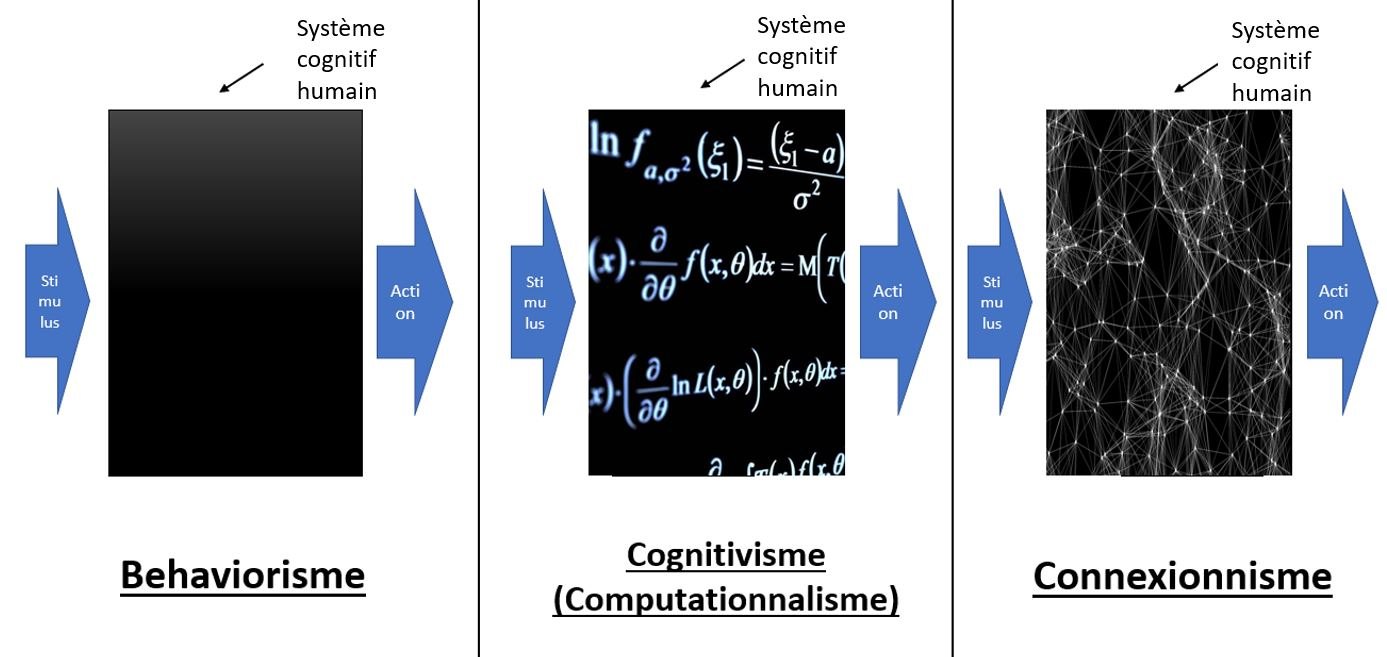
\includegraphics[scale=0.3]{imgs/1.JPG}
\caption{Illustration schématique du système cognitif humain dans certaines approches d'étude de la cognition humaine}
\end{figure}

\pagebreak

	\textbf{Apparté : Motivation personnelles}

	 C'est donc avec ces idées (celles énoncées dans l'introduction pour ceux qui lisent dans le désordre) que j'aborde ce Travail Encadré de Recherche dans le cadre de ma troisème année de licence de Mathématiques et Informatique appliquées aux sciences humaines et sociales - Parcours Sciences Cognitives à l'université de Bordeaux. Ce TER a, je dois bien l'avouer, surtout une portée d'apprentissage pour moi, puisque j'espère qu'il me permettra d'acquérir les connaissances necessaire sur la modélisation du système nerveux pour ensuite poursuivre les buts énoncés dans l'introduction dans la suite de mes études, puis en recherche. Pour justifier la création de mes propres outils de définition et de simulation des modèles, je dirais que cela me permettra une compréhension profonde de la manière dont fonctionnent ces outils, notamment des méthodes de simulation numérique. De plus, il y a un manque d'outil de création de réseaux de spiking neurons en Python, et je pense que l'utilisation de tensorflow (bibliothèque de computation parallèle et optimisée) se revelera pertinente, et j'espère ainsi, au cours de ce travail et après, créer une bibliothèque de création de modèles de réseaux de neurones biologiques facile d'utilisation et optimisée en terme de computation, du moins autant que cela est possible. Enfin l'étude et la reproduction des travaux de Héricé et all 2016 permettront, en plus de m'apporter de la connaissance et de la pratique sur la base d'une partie de la littérature récente sur le sujet, d'apporter une justification de l'utilité de mon outil de simulation de réseaux de neurones.

\pagebreak

\part{Modélisation d'un neurone}
\section{Quelques rappels de neurobiologie}
	Cette partie sera concise et aura pour but de rappeler quelques notions de neurobiologie necessaire à la compréhension de la suite, sans en faire trop. On suppose que le lecteur est déjà familier avec les notions fondamentales de la neurobiologie, si ce n'est pas le cas, on renvoie à Principles of Neural Science de Eric Kandel.  
Le neurone est une cellule capable de recevoir et transmettre de l'information sous forme electro-chimique. On peut décomposer schématiquement les différentes étapes de la reception et transmition de l'information in vivo dans un neurone par :
\begin{enumerate}
	\item Reception de neurotransmetteurs et ouverture des canaux chimio-dépendants
	\item Excitation electrique locale du neurone dû à l'ouverture des canaux chimio-dépedants
	\item Lorsque l'excitation locale depasse un certain seuil, création d'un potentiel d'action
	\item Transmition du potentiel d'action à travers l'axone
	\item Libération de neurotransmetteur dans la fente synaptique dû à l'arrivée du potentiel d'action dans le bouton synaptique 
	\item Repeter 1. pour le neurone post-synaptique
\end{enumerate}

	Lorsqu'on souhaite étudier les propriétés d'excitation d'un neurone en laboratoire, on va généralement provoquer l'excitation du neurone en injectant directement un courant electrique dans le neurone, et on va s'interesser à la production de potentiels d'action en fonction des propriétés du courant injecté, notamment de son intensité (technique de patch-clamp). 

	Dans cette idée d'étude de la production de potentiel d'action en fonction des propriétés d'un courant injecté directement dans le neurone, on ne décrira pas ici les mécanismes à l'oeuvre dans la synapse.

	Le concept fondamental de neurobiologie en lien avec cette partie est celui de la création du potentiel d'action. On rappellera ici succintement les mecanismes neurobiologiques à l'oeuvre. On peut décomposer la génération d'un potentiel d'action en 5 phases :
	\begin{enumerate} \item Dépolarisation faible : ouverture de certain canaux sodiques, entrée des ions sodium dans le milieu intracellulaire ;
	\item Dépolarisation forte suite au dépassement de seuil : Lorsqu'un certain seuil de potentiel electrique est atteint (le potentiel de seuil), la membrane va subir une dépolarisation forte, allant jusqu'à un inversement de polarité où le potentiel de la membrane est d'environ 40 mV. Cette dépolarisation est due à l'ouverture massive de canaux sodiques. Une fois le changement de polarité effectué, l'inversion du gradient electrochimique va ralentir l'entrée des ions sodium dans la cellule ;
	\item Repolarisation : L'ouverture des canaux potassiques et l'inactivation des canaux sodiques entraine la sortie massive d'ions potassium et un arret de l'entrée des ions sodium;
	\item Hyperpolarisation : En continuité de la repolarisation, on observe que le potentiel membranaire ne revient pas directement au potentiel de repos, mais passe sous le potentiel de repos pendant un certain temps que l'on appelle la période refractaire. Cela est du au fait que les canaux potassiques restent ouverts plus longtemps que les canaux sodiques, on a donc une sortie d'ions K+ plus importante que necessaire pour revenir au potentiel de repos;
	\item Retour au potentiel de repos : Le retour au potentiel de repos est assuré par la pompesodium/potassium.
	\end{enumerate}

\begin{figure}[!h]
\centering
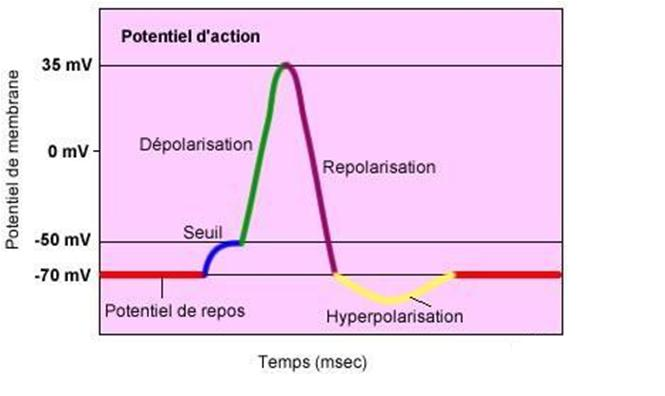
\includegraphics{imgs/2.JPG}
\caption{Potentiel de la membrane en fonction du temps lors de la production d'un potentiel d'action}
\end{figure}

\section{Modele de Hodgkin Huxley}\label{hh}
	L'approche de Hodgkin et Huxley sur la question de la modélisation de neurones est une approche qui possède une grande "clarté physiologique", dans le sens où chaque composante du modèle représente une réalité biologique ou electrique descriptible dans les termes de la neurobiologie. On peut ainsi attribuer au modèle de Hodgkin-Huxley une certaine cohérence et validité par rapport aux sciences naturelles (notamment neurobiologie encore une fois). Mais voyons ça plus en détails ..
	
	\subsection{La modélisation des canaux ioniques}
		Comme nous l'avons rapellé dans 2., la génération de potentiels d'actions est gouvernée, au niveau moléculaire, par les dynamiques d'ouverture et de fermeture des canaux ioniques. Ces canaux peuvent être dans différents états : ouverts ou fermés, bien sur, mais aussi actifs ou inactifs, et il est necessaire qu'un canal soit à la fois dans l'état ouvert et actif pour que les ions puissent passer. Hodgkin-Huxley ont fait 2 hypothèses sur ces canaux ioniques dans leur travaux, sur la base d'observation des neurones biologiques : Premièrement, la génération du potentiel d'action est gouvernée par les mouvements des ions potassium et sodium, et pas des autres ions, et deuxièmement, les canaux sodiques et potassique sont divisés en différentes composantes. Les canaux potassiques se divisent en 4 composantes équivalentes qui gouverne l'ouverture du canal : le canal est ouvert lorsque les 4 composantes sont ouvertes. Les canaux potassiques étant de plus considérés comme toujours actif, le passage des ions est permit lorsque ces 4 composantes sont ouvertes. Les canaux sodiques, quand à eux, se divisent en 3 composantes gouvernant l'ouverture du canal, et 1 composante gouvernant l'activation du canal. Il est necessaire que les 3 composantes gouvernant l'ouverture soient ouvertes et que la composante gouvernant l'activation du canal soient active pour que les ions puissent passer dans le canal.

On notera $n \in [0, 1]$ la probabilité qu'une composante d'un canal potassique soit ouverte, et donc $(1-n)$ est la probabilité que la composante soit fermée. On sait que l'ouverture et la fermeture de ces canaux ioniques dépend du potentiel de membrane, ainsi, on a $\alpha_n$ et $\beta_n$ des fonctions du potentiel qui définissent respectivement le passage de l'état fermé  à l'état ouvert, et de l'état ouvert à l'état fermé. Si on connait la probabilité initale $n(t_0)$ que la composante soit ouverte en $t_0$, on peut déduire la probabilité que la composante soit ouverte pour tout $t$. En effet, la probabilité qu'une composante soit ouverte pendant $dt$ est la probabilité qu'on soit fermeé et qu'on passe de l'état fermée à l'état ouvert moins la probabilité qu'on soit ouvert et qu'on passe de l'état ouvert à l'état fermée. Ainsi, 
\begin{center} $\displaystyle \frac{\dd n}{\dd t} = \alpha_n(V)(1-n) - \beta_n(V) n$ \end{center}
Et on peut réécrire cette question sous la forme :
\begin{center} $\displaystyle \tau_n \frac{\dd n}{\dd t} = n_{\infty} - n$ \end{center}
avec $\tau_n = \frac{1}{\alpha_n+\beta_n}$ la constante de temps et $n_\infty = \frac{\alpha_n}{\alpha_n+\beta_n}$ la valeur de n à l'équilibre. \\
Etant donné qu'il est nécessaire que les quatre composantes du canal soient ouvertes pour que le canal soit lui-même "ouvert", c'est-à-dire qu'il laisse passer les ions, la probabilités que le canal soit ouvert est la probabilité que les quatre composantes soient ouvertes, soit $n^4$.

Maintenant que nous avons définit les variations de la probabilité d'ouverture des canaux potassiques, nous allons faire de même pour les canaux sodiques. La différence ici par rapport au canal potassique est qu'il faut prendre en compte, en plus de l'ouverture et de la fermetture, l'activation et l'inactivation du canal. On devra donc utiliser deux probabilité différentes : $m \in [0,1]$ la probabilité qu'une composante controlant l'ouverture soit ouverte (et donc $(1-m)$ est la probabilité que la composante soit fermée) et $h \in [0,1]$ la probabilité que le canal soit actif (et donc $(1-h)$ la probabilité qu'il soit inactif). Etant donné que l'activation et l'inactivation n'est controlée que par une seule composante, l'activation ou l'inactivation de cette composante est equivalente à l'activation ou l'inactivation du canal. On définit $\alpha_m, \beta_m, \alpha_h, \beta_h$ les fonctions du potentiel qui définissent respectivement le passage de l'état fermé à l'état ouvert d'une composante controlant l'ouverture, le passage de l'état ouvert à l'éta fermé d'une composante controlant l'ouverture, le passage de l'état inactif à l'état actif du canal, le passage de l'état actif à l'état inactif du canal. Et, de la même manière que pour les canaux potassiques, on a les équations 
\begin{center} $\displaystyle \frac{\dd m}{\dd t} = \alpha_m(V)(1-m) - \beta_m(V) m$ \end{center}
\begin{center} $\displaystyle \frac{\dd h}{\dd t} = \alpha_h(V)(1-h) - \beta_h(V) h$ \end{center}
Que l'on peut réécrire comme ceci :
\begin{center} $\displaystyle \tau_m \frac{\dd m}{\dd t} = m_{\infty} - m$ \end{center}
\begin{center} $\displaystyle \tau_h \frac{\dd h}{\dd t} = h_{\infty} - h$ \end{center}
avec encore une fois $\tau_m = \frac{1}{\alpha_m+\beta_m},~\tau_h = \frac{1}{\alpha_h+\beta_h} $ les constantes de temps et \\$m_\infty = \frac{\alpha_m}{\alpha_m+\beta_m},~h_\infty = \frac{\alpha_h}{\alpha_h+\beta_h}$ les valeurs de m et h à l'équilibre. \\
Ici, il est nécessaire que le canal soit actif et que les trois composantes controlant l'ouverture soient ouvertes pour que le canal laisse passer les ions, ainsi la probabilité que le canal laisse passer les ions est $m^3h$.

En plus des ces équations qui permettent de connaitre la probabilité qu'un canal soit ouvert au temps t, on va également définir les conductances d'un canal lorsqu'il est ouvert et le potentiel d'équilibre associé à chaque ion. On notera $\overline{g}_{Na}$ et $\overline{g}_K$ les conductances associées respectivement aux ions sodium et potassium, et $V_{Na}$ et $V_K$ les potentiels d'équilibre donné par la formule de Nerst pour respectivement les ions sodium et potassium.

Pour finir, Hodgkin et Huxley ont également introduit dans leur modèle un "courant de fuite", c'est-à-dire un courant qui modélise l'impact de tous les échanges d'ions qui ne sont pas gouvernés par les canaux sodium et potassium. On va donc définir en plus $\overline{g}_L$ et $V_L$ respectivement la conductance et le potentiel d'equilibre associée à ce courant de fuite.

\pagebreak
	\subsection{L'équation du potentiel de membrane}
Il est possible de représenter un neurone dans le modèle de Hosgkin-Huxley comme un circuit electrique (voir \ref{HHFIG}). Dans cette représentation, on peut assimiler le condensateur à la bicouche lipidique isolante de la membrane, la résistance aux passages des ions à travers la membrane, et la pile aux gradient de concentration. Grace à cette représentation, il est plus facile d'expliquer l'équation représentant les variations du potentiel de membrane du neurone. On va ici en faire une explication intuitive en se basant sur des grands principes issus des sciences physiques :
\begin{itemize}
\item Loi d'Ohm 
\item loi de Kirchoff
\item definition d'un capaciteur 
\item dérivée de la charge par rapport au temps = intensité, 
\end{itemize}
applications pour trouver l'eq, système d'eq en entier.

\begin{figure}[!h]
\centering
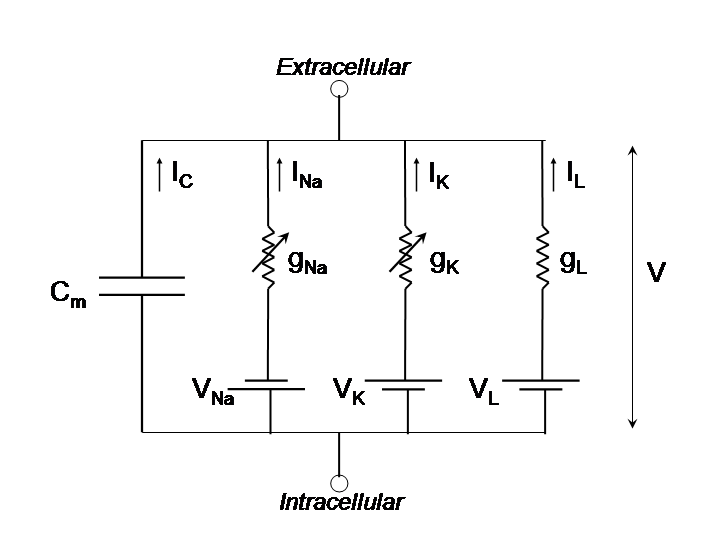
\includegraphics[scale=0.5]{imgs/3.png}
\caption{Représentation du modèle de Hodgkin-Huxley sous forme d'un circuit electrique}
\label{HHFIG}
\end{figure}

	\subsection{Simulation avec SNN.single et explication des dynamiques}

On va simuler le modèle de Hodgkin-Huxley à l'aide de l'outil informatique que nous avons mis en place. Certains graphiques ne seront pas expliqués et leur interprétation sera laissé au lecteur.

Pour simuler numériquement le modèle, il faut avoir des valeurs pour $C_M$, les conductances $\overline{g}_X$, les potentiels d'équilibre $V_X$, et les fonctions $\alpha_X$ et $\beta_X$.
En tentant de rapprocher les comportements du modèle de données phyiologiques recoltées à l'aide de la technique de patch-clamp (originellement dans les travaux de Hodgkin-Huxley sur un axone de calamar, ayant la particularité d'être très gros), on trouve les valeurs pour les paramètres : \\\\
$ C_M = 1,~ \overline{g}_K = 36,~ \overline{g}_{Na} = 120,~ \overline{g}_L = 0.3,~ V_K = -77,~ V_{Na} = 50,~ V_L = -54.4,\\\\
\alpha_n(V) =\frac{ 0.01(-V-55)}{\e^{\frac{-V-55}{10}}-1},~ \beta_n=0.125e^{\frac{-V-65}{80}}\\\\
\alpha_n(V) =\frac{ 0.1(-V-40)}{\e^{\frac{-V-40}{10}}-1},~ \beta_n=4e^{\frac{-V-65}{18}}\\\\
\alpha_n(V) =0.07e^{\frac{-V-65}{20}},~ \beta_n=\frac{1}{1+e^{\frac{-V-35}{10}}}$

\begin{lstlisting}[caption = {Défintion du modèle}]
from .core import Variable, Model
from .tools import Function as F

V = Variable(name='V', init_value=-65,
		ddt='(1/Cm)*(-gk*n**4*(V-Vk)-gna*m**3*h*(V-Vna)-gl*(V-Vl)+Iapp)')
n = Variable(name='n', ddt='alpha_n*(1-n)-beta_n*n', init_value=1/3)
m = Variable(name='m', ddt='alpha_m*(1-m)-beta_m*m', init_value=0)
h = Variable(name='h', ddt='alpha_h*(1-h)-beta_h*h', init_value=2/3)
HH_model = Model(V, n, m, h, Cm=1, gk=36, gna=120, 
				 gl=0.3, Vk=-77, Vna=50, Vl=-54.4, 
				 alpha_n=F('V', lambda V: 0.01*(-V-55)/(e**((-V-55)/10) -1)), 
				 beta_n=F('V', lambda V: 0.125*e**((-V-65)/80)),
				 alpha_m=F('V', lambda V: 0.1*(-V-40)/(e**((-V-40)/10) -1) ),
				 beta_m=F('V', lambda V: 4*e**((-V-65)/18)),
				 alpha_h=F('V', lambda V: 0.07*e**((-V-65)/20)),
				 beta_h=F('V', lambda V: 1/(1+e**((-V-35)/10))), 
				 Iapp=0)
\end{lstlisting}

\begin{lstlisting}[caption = {Simulation du modèle 1}]
import math
import random as rd 
from snn.single.tools import Function as F
from snn.single.usual_models import HH_model as hh
import matplotlib.pyplot as plt

# Define Input current
hh['Iapp'] = 5
# Runge-Kutta method for numerical simulation
hh.method = 'rk4'

# Since we are plotting multiple things, it's better to simulate the
# model only one time, and then feed the results to the plot method
T, dt = 100, 0.01
history, _ = hh.simulation(T, dt)

# Plot the input current and the membrane 
# potential evolution throught time
fig1 = hh.plot(T, dt, keep=['V', 'Iapp'], history=history)

# Print m, n, h evolution when the membrane potentiel changes
fig3 = plt.figure() ; plt.ylabel('n'), plt.xlabel('V')
plt.plot(history['V'], history['n'])
fig4 = plt.figure() ; plt.ylabel('m'), plt.xlabel('V')
plt.plot(history['V'], history['m']) 
fig5 = plt.figure() ; plt.ylabel('h'), plt.xlabel('V')
plt.plot(history['V'], history['h']) 

plt.show()
\end{lstlisting}



\begin{figure}[!h]
\centering
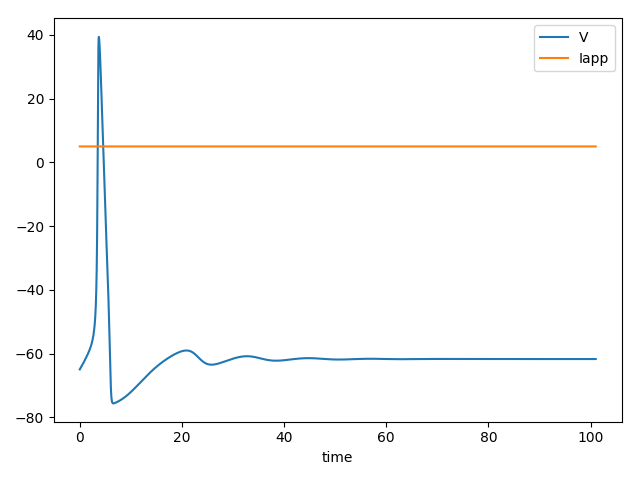
\includegraphics[scale=0.5]{imgs/hh11.png}
\caption{Evolution du courant appliqué et du potentiel de membrane au cours du temps}
\label{hh11}
\end{figure}

\begin{figure}[!h]
\begin{minipage}[l]{.3\linewidth}
\centering
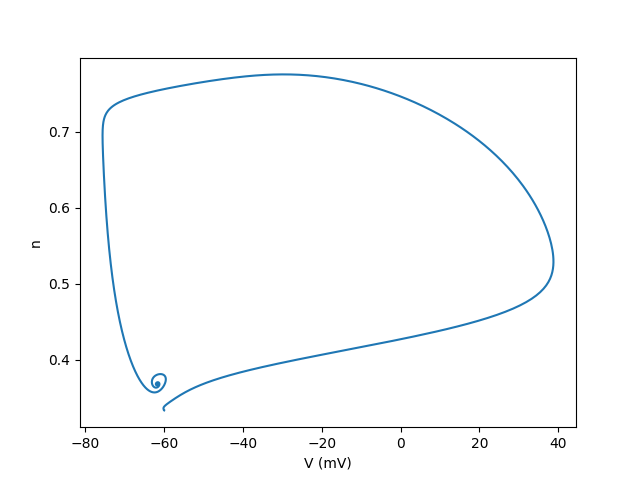
\includegraphics[scale=0.35]{imgs/hh12.png}
    \end{minipage}\hfill
\begin{minipage}[l]{.3\linewidth}
\centering
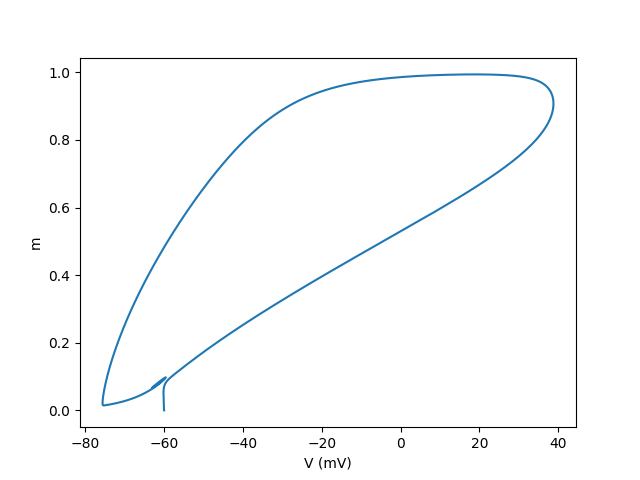
\includegraphics[scale=0.35]{imgs/hh13.png}
    \end{minipage}\hfill
\begin{minipage}[l]{.3\linewidth}
\centering
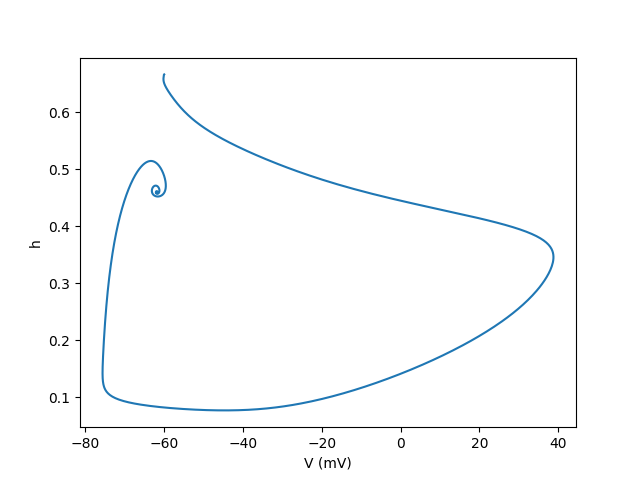
\includegraphics[scale=0.35]{imgs/hh14.png}
    \end{minipage}\hfill
\caption{n, m et h en fonction de v}
\label{hh1234}
\end{figure}

\clearpage

\begin{lstlisting}[caption = {Simulation du modèle 2}]
hh['Iapp'] = 10
T, dt = 100, 0.01
\end{lstlisting}

\begin{figure}[!h]
\centering
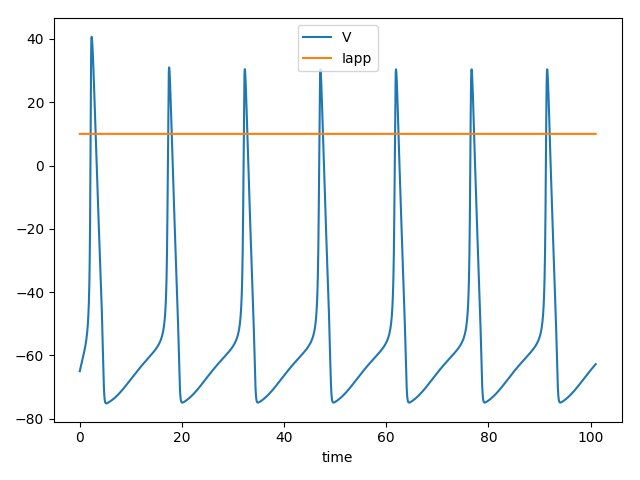
\includegraphics[scale=0.4]{imgs/hh21.png}
\caption{Evolution du courant appliqué et du potentiel de membrane au cours du temps}
\label{hh21}
\end{figure}

\begin{figure}[!h]
\begin{minipage}[l]{.3\linewidth}
\centering
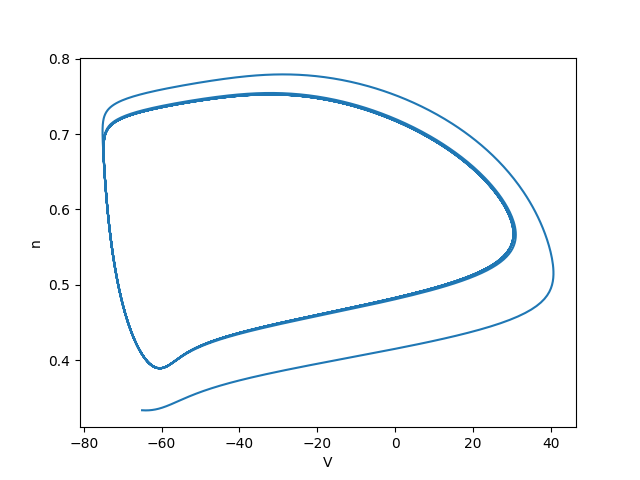
\includegraphics[scale=0.35]{imgs/hh22.png}
    \end{minipage}\hfill
\begin{minipage}[l]{.3\linewidth}
\centering
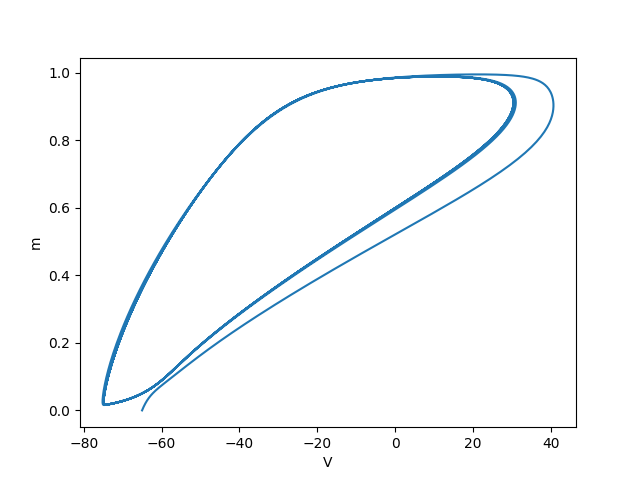
\includegraphics[scale=0.35]{imgs/hh23.png}
    \end{minipage}\hfill
\begin{minipage}[l]{.3\linewidth}
\centering
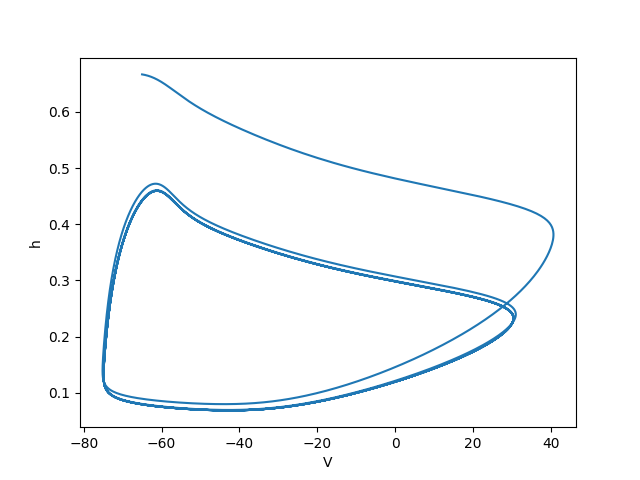
\includegraphics[scale=0.35]{imgs/hh24.png}
    \end{minipage}\hfill
\caption{n, m et h en fonction de v}
\label{hh2234}
\end{figure}

Dans \ref{hh11}, on peut voir que le modèle est bien capable de produire un potentiel d'action, en tout cas le comportement de la variable V représentant le potentiel de membrane a un comportement similaire aux potentiel de membrane \textit{in vivo}. Le courant appliqué, qui est constant égal à 5, est suffisant pour provoquer un potentiel d'action mais insuffisant pour en provoquer un deuxième. Au contraire, dans \ref{hh21}, le courant constant égal à 10 est suffisant pour provoquer un train de potentiel d'action, à partir du deuxième potentiel d'action, on a un comportement périodique du système, qui va continuer de générer des potentiels d'action si le courant appliqué reste constant. Cela peut également se voir sur les représentations de m, n et h en fonction de V. Lorsqu'il n'y a qu'un seul potentiel d'action puis une convergence vers un état stable , on peut voir dans \ref{hh1234} la présence d'un équilibre attracteur pour m, n et h, ce qui signifie que l'état du système va se stabiliser. Au contraire, lorsqu'on a une génération périodique de potentil d'action comme dans \ref{hh2234}, on voit bien que le comportement de m, n et h est cyclique et qu'il n'y a pas d'équilibre attracteur.\\\\\\

\begin{lstlisting}[caption = {Simulation du modèle 3}]
hh['Iapp'] = F('t', 
								lambda t : 5 if 200<t<400 else 10 if 600<t<800 else 0)
T, dt = 1000, 0.01
\end{lstlisting}

\begin{figure}[!h]
\centering
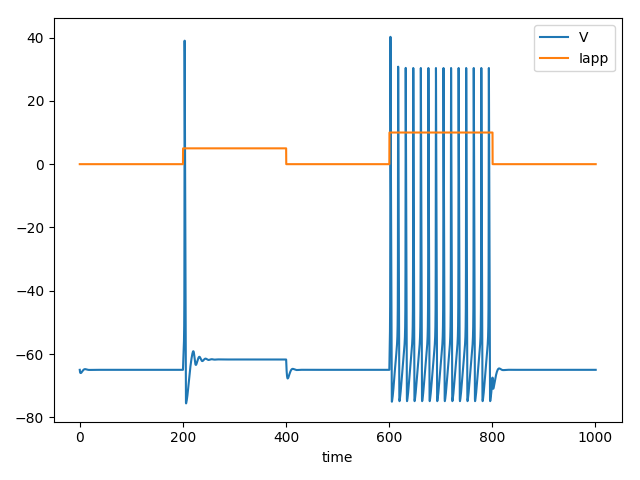
\includegraphics[scale=0.8]{imgs/hh31.png}
\caption{Evolution du courant appliqué et du potentiel de membrane au cours du temps}
\label{hh31}
\end{figure}

\clearpage
\begin{lstlisting}[caption = {Simulation du modèle 4}]
hh['Iapp'] = F('t', lambda t : 5*math.cos(t/10) + rd.expovariate(0.5))
T, dt = 100, 0.01
\end{lstlisting}

\begin{figure}[!h]
\centering
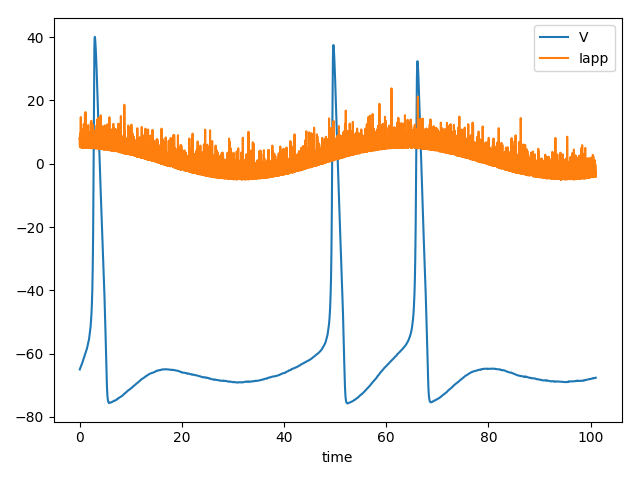
\includegraphics[scale=0.8]{imgs/hh41.png}
\caption{Evolution du courant appliqué et du potentiel de membrane au cours du temps}
\label{hh41}
\end{figure}

\clearpage 
\begin{lstlisting}[caption = {Simulation du modèle 5}]
hh['Iapp'] = 10
T, dt = 12, 0.01
fig2 = hh.plot(T, dt, keep=['m', 'n', 'h'], #subplotform='31', 
			 history=history)
\end{lstlisting}

\begin{figure}[!h]
\centering
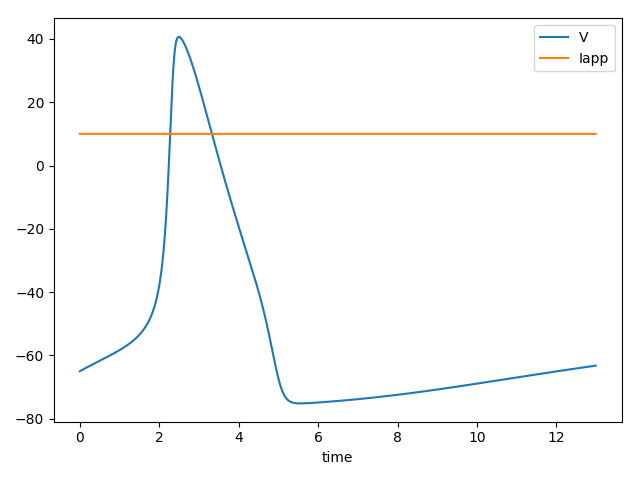
\includegraphics[scale=0.5]{imgs/hh51.png}
\caption{Evolution du courant appliqué et du potentiel de membrane au cours du temps}
\label{hh51}
\end{figure}

\begin{figure}[!h]
\centering
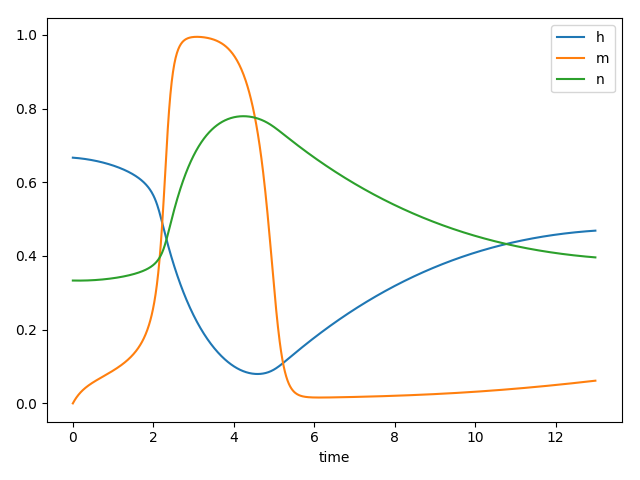
\includegraphics[scale=0.5]{imgs/hh52.png}
\caption{Evolution des paramètres m, n et h lors de la génération d'un potentiel d'action}
\label{hh52}
\end{figure}

\clearpage

\begin{lstlisting}[caption = {Simulation du modèle 4}]
hh['Iapp'] = 10
T, dt = 12, 0.01

#Plotting time constant
plt.figure()
plt.plot(history['V'], 1/(history['alpha_n']+history['beta_n']),
	label='\u03C4_n')
plt.plot(history['V'], 1/(history['alpha_m']+history['beta_m']),
	label='\u03C4_m')
plt.plot(history['V'], 1/(history['alpha_h']+history['beta_h']),
	label='\u03C4_h')
plt.legend()

#Plotting equilibrium state
plt.figure()
plt.plot(history['V'],
	history['alpha_n']/(history['alpha_n']+history['beta_n']),
	label='n_\u221E')
plt.plot(history['V'],
	history['alpha_m']/(history['alpha_m']+history['beta_m']),
	label='m_\u221E')
plt.plot(history['V'],
	history['alpha_h']/(history['alpha_h']+history['beta_h']),
	label='h_\u221E')
plt.legend()

plt.show()
\end{lstlisting}

\begin{figure}[!h]
\centering
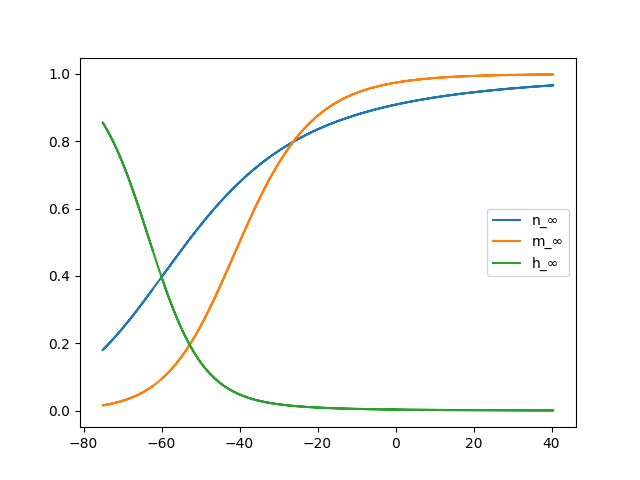
\includegraphics[scale=0.5]{imgs/hhinfty.png}
\caption{Evolution des paramètres $n_\infty$, $m_\infty$ et $h_\infty$ lors de la génération d'un potentiel d'action}
\label{hhinfty}
\end{figure}

\begin{figure}[!h]
\centering
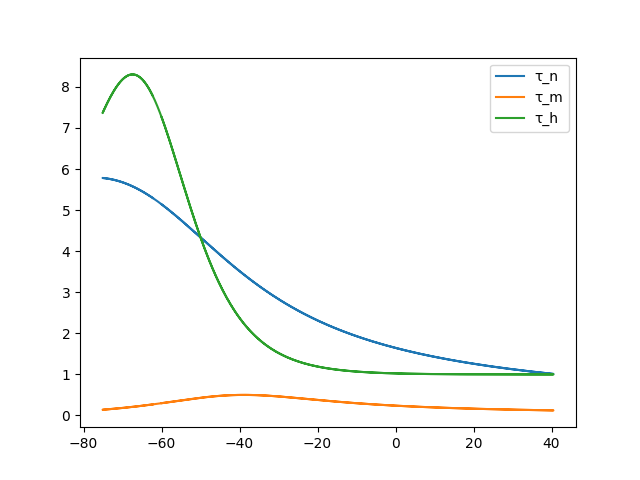
\includegraphics[scale=0.5]{imgs/hhtime.png}
\caption{Evolution des paramètres $\tau_n$, $\tau_m$, $\tau_h$ lors de la génération d'un potentiel d'action}
\label{hhtime}
\end{figure}

\clearpage
\textbf{Explication des dynamiques à partir des constantes de temps et des valeurs à l'équilibre}\\
De \ref{hhinfty}, on peut tirer le fait que n et m sont croissants par rapport au potentiel, tandis que h est décroissant par rapport au potentiel. Ainsi, les canaux poassiques vont avoir une probabilité de laisser passer les ions de plus en plus grande plus le potentiel augmente, tandis que pour les canaux sodiques, leur probabilité de laisser passer les ions va d'abord augmenter quand le potentiel augmente (du au fait que m est croissante par rapport au potentiel), puis, à partir d'un certain seuil, diminuer quand le potentiel augmente (du  au fait que h est décroissante par rapport au potentiel).\\
Les constantes de temps, qui gouvernent la temps que met le système à atteindre les valeurs à l'équilibre, sont également intéressantes à étudier pour comprendre les dynamiques à l'oeuvre. On peut voir dans \ref{hhtime}, que m, qui gouverne l'ouverture des canaux sodique, atteint très rapidement sont état d'équilibre, tandis que n (ouverture des canaux potassiques) et h(activation des canaux sodiques) l'atteignent plus lentement.\\
Ainsi, lorsque la membrane est dépolarisée, la variable m va augmenter (vers son etat d'équilibre) rapidement (les canaux sodiques vont s'ouvrir rapidement), ce qui va en retour augmenter la dépolarisation de la cellule (le potentiel de membrane va tendre vers $V_{Na}$), et m va de nouveau augmenter, etc .. Avec un délai du aux dynamiques (c'est-à-dire ici au temps d'atteinte de la valeur d'équilibre) plus lentes de h et n, on va observer que h va diminuer (tendre vers sa valeur d'équilibre)(les canaux sodiques vont être désactivés), et de plus, n va augmenter (tendre vers sa valeur d'équilibre)(les canaux potassiques vont s'ouvrir), ce qui aura pour effet de repolarisée la cellule (le potentiel de membrane va tendre vers $V_{K}$). La période refractaire, c'est-à-dire l'hyperpolarisation de la membrane peut s'expliquer par le délai dans le retour à un état d'équilibre de la variable n (les canaux potassiques se referment avec un délai).


\section{Raffiner Hodgkin-Huxley}
\subsection{Les deux approches possibles face à Hodgkin-Huxley}
	Les travaux de Hodgkin et Huxley abordé en \ref{hh} ont véritablement révolutionné le domaine de la modélisation de neurones, et depuis, une grande partie des travaux en modélisation de neurones s'appuien sur ceux de Hodgkin et Huxley. Les scientifiques s'interessant  à la modélisation de neurones ont pu avoir deux grandes approches (ces deux grandes approches pouvant s'étendre à tous les travaux en modélisation de neurones, et pas seulement à ceux se basant sur le modèle de Hodgkin et Huxley) : 
		\begin{enumerate} \item \textbf{Complexifier Hodgkin-Huxley : Reproduire le plus fidélement possible un neurone ou un réseau de neurone sans se soucier de la complexité du modèle}, ce qui donne un modèle plus précis, plus proche de la réalité, mais difficilement manipulable et compréhensible, et dont la simulation est couteuse (en temps). On retrouve dans cette catégorie la plupart des modèles dit "physiologiques", c'est-à-dire les modèles qui s'inspirent du fonctionnement biologique du système nerveux et tentent de le formaliser.  
		\item \textbf{Simplifier Hodgkin-Huxley : Faire un compromis entre le réalisme du modèle et sa complexité}, ce qui donne des modèles moins précis et moins proche de la réalité, mais plus facilement manipulable, compréhensible et dont la simulation est rapide. On retrouve dans cette catégorie la plupart des modèles dit "phénoménologiques", c'est-à-dire les modèles qui, sans la contrainte de s'inspirer du biologique, tentent de reproduire le fonctionnement du système nerveux en terme de données quantitatives "de plus haut niveau", comme par exemple le potentiel de membrane d'un neurone. \end{enumerate}
Un modèle de neurone théorique parfait devrai posséder les qualités des deux approches sans posséder leur défauts ... mais cela semble pour l'instant impossible. Le réalisme passe par la complexité du modèle, et la complexité du modèle entraine que la simulation informatique et que l'explication mathématique seront couteuses. Ainsi, lorsque l'on doit choisir un modèle de neurone, on doit le faire dans objectif précis, et il est important de bien comprendre quelles sont les caractéristiques du modèle importantes pour réaliser notre objectif. Dans le cas de ce travail, nous allons par la suite vouloir réaliser des simulations de réseaux de grandes tailles de manière rapide, répétable. C'est ainsi, et c'est un choix de notre part, que nous allons ici plutot nous interesser aux modèles simples, venant de l'approche 2., pour leur simplicité et rapidité de simulation. 

\subsection{De Hodgkin-Huxley à Fitzhugh-Nagumo, et explication de Fitzhugh-Nagumo}

\subsection{De Fitzhugh-Nagumo à Izhikievich, explication et démonstration de la puissance du modèle de Izhikievich}
	A partir d'une analyse du plan de phase du modèle de Fitzhugh-Nagumo, on peut remarquer que, dans la région du plan de phase responsable de la génération des potentiels d'actions, la V-isocline peut se résumer

\section{Modèle leaky-integrate and fire}
	Encore plus simple : le modèle leaky-integrate and fire, présentation du modèle, explications, simulations.


\section{Quelques mots sur les modeles compartimentaux et augmentation de Hodkin-Huxley}\label{hhcomplex}
	Principe (approximation des différentes composantes par des cylindres) et équation du cable. Interets ( biologiquement + réaliste). Techniques de réduction du nombre de compartiments avec same beahvior. 

\nocite{*}

\pagebreak

\part{Réseau de neurones}

\part{Etude de (Héricé et al., 2016) }

\part{Code}
\url{https://github.com/ArnoGranier/SNN}

Quelques justifications informatiques :
\begin{itemize} \item Cette partie informatique de création d'outils de simulation ayant une grande par didactique pour moi, j'ai souhaité dans la partie de modélisation d'un seul neurone, ne pas utiliser certains outils "déjà tout pret" et plutot coder moi-même un maximum de chose. C'est la raison pour laquel je n'utilise numpy que pour retourner des types array et que je n'utilise pas les méthodes linspace ou meshgrid (par exemple) de cette bibliothèque. J'ai également souhaté ne pas utiliser d'ODE-solver djà implémenté comme on peut trouver dans scipy.integrate par exemple. \end{itemize}


\bibliographystyle{apacite}
\bibliography{ref}




\end{document}

